\documentclass[12pt]{article}
\usepackage[utf8]{inputenc}
\usepackage{tgbonum}
\usepackage[a4paper, total={7in, 10in}]{geometry}
\usepackage{graphicx}
\usepackage{minted}
\title{Lab Assignment 7}
\author{Akshat Mittal - 20107}
\date{July 2021}
\begin{document}
\maketitle
\vspace{7mm}
\textbf{Contents}
\vspace{7mm}
\begin{enumerate}
    \item Customers in a bank
    \item Comparing Dates
    \item Student Details Management
    \item Library Management
    \item Structures and functions
    \item Party Items
    \item Employee Management
    \item Unions in C
    \item Union in substitute of structure
    \item Unions and floats
\end{enumerate}

\newpage
\section{}
\subsection{Code}
\inputminted{c}{q1.c}
\subsection{Output}
\begin{figure}[h]
    \centering
    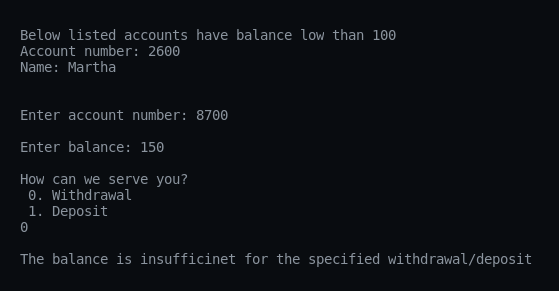
\includegraphics[width=1\textwidth]{1.png}
\end{figure}

\newpage
\section{}
\subsection{Code}
\inputminted{c}{q2.c}
\newpage
\subsection{Output}
\begin{figure}[h]
    \centering
    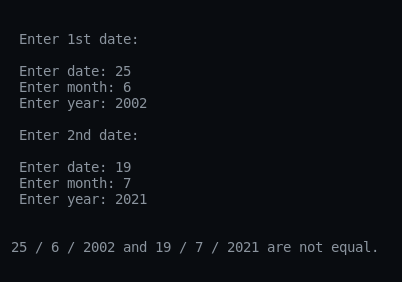
\includegraphics{2.png}
\end{figure}

\newpage
\section{}
\subsection{Code}
\inputminted{c}{q3.c}
\newpage
\subsection{Output}
\begin{figure}[h]
    \centering
    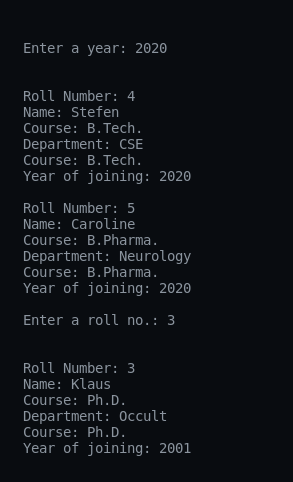
\includegraphics[width=0.65\textwidth]{3.png}
\end{figure}

\newpage
\section{}
\subsection{Code}
\inputminted{c}{q4.c}
\newpage
\subsection{Output}
\begin{figure}[h]
    \centering
    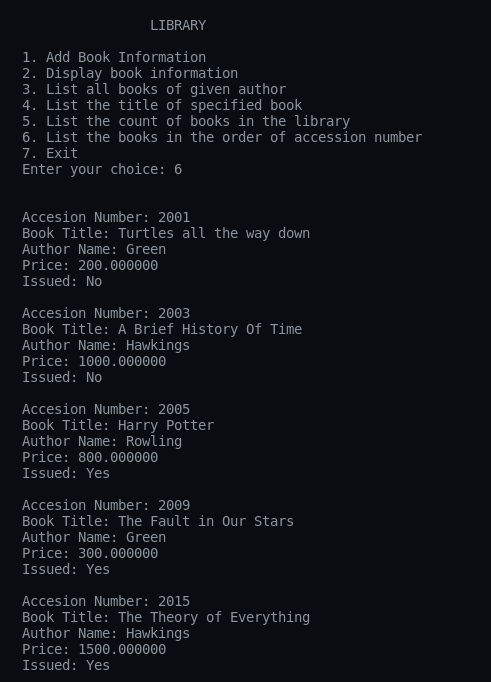
\includegraphics[width=0.8\textwidth]{4.png}
\end{figure}

\newpage
\section{}
\subsection{Code}
\inputminted{c}{q5.c}
\newpage
\subsection{Output}
\begin{figure}[h]
    \centering
    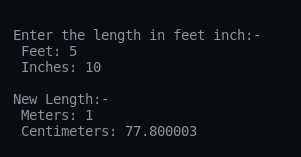
\includegraphics[width=0.8\textwidth]{5.png}
\end{figure}

\newpage
\section{}
\subsection{Code}
\inputminted{c}{q6.c}
\newpage
\subsection{Output}
\begin{figure}[h]
    \centering
    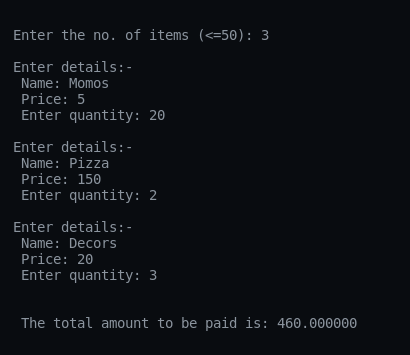
\includegraphics[width=0.8\textwidth]{6.png}
\end{figure}

\newpage
\section{}
\subsection{Code}
\inputminted{c}{q7.c}
\subsection{Output}
\begin{figure}[h]
    \centering
    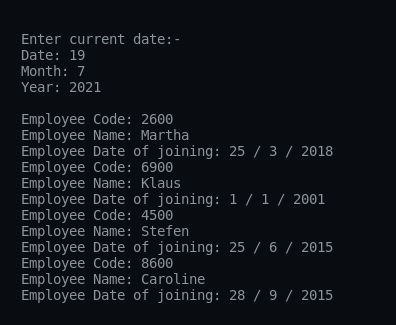
\includegraphics[width=0.8\textwidth]{7.png}
\end{figure}

\newpage
\section{}
\subsection{Code}
\inputminted{c}{q8.c}
\subsection{Output}
\begin{figure}[h]
    \centering
    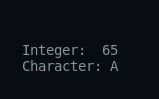
\includegraphics[width=0.6\textwidth]{8.png}
\end{figure}
\newpage
\section{}
\subsection{Code}
\inputminted{c}{q9a.c}
\subsection{Output}
\begin{figure}[h]
    \centering
    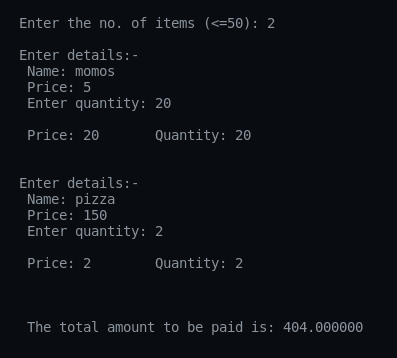
\includegraphics[width=0.75\textwidth]{9a.png}
\end{figure}
\newpage
\subsection{Code}
\inputminted{c}{q9b.c}
\subsection{Output}
\begin{figure}[h]
    \centering
    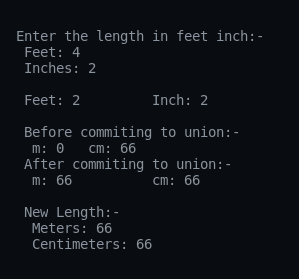
\includegraphics[width=0.7\textwidth]{9b.png}
\end{figure}
\newpage
\section{}
\subsection{Code}
\inputminted{c}{q10.c}
\subsection{Output}
\begin{figure}[h]
    \centering
    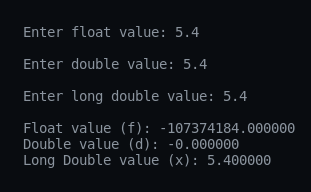
\includegraphics[width=0.75\textwidth]{10.png}
\end{figure}

\end{document}